\documentclass{article}
\usepackage[utf8]{inputenc}
\usepackage{amssymb}
\usepackage{tikz}
\usepackage{amsmath}
\usepackage{relsize}
\usepackage{mathtools}
\usepackage{textcomp}
\usepackage{eurosym}
\usepackage{amssymb}
\usepackage{systeme}
\usepackage{mathtools}
\usepackage{graphicx}
\usepackage{subfig}
\usepackage[bottom]{footmisc}
\usepackage{mwe}

\title{Method}
\author{Roman Oort}
\date{\today}

%%% PERSONAL SHORTCUTS
\DeclareMathOperator*{\plim}{plim}
\newcommand{\T}{\textbf{T}}
\newcommand{\Tij}{\textbf{T}_{ij}}
\newcommand{\Soc}{(\T(n))^{\infty}_{n=1}}
\newcommand{\beli}[3][2]{p_{#2}^{(#3)}}
\newcommand{\belvec}[2]{\textbf{p}^{(#2)}}

\begin{document}

\maketitle

\tableofcontents
\newpage
\section{Network Generation}

\subsection{Random Generation}

In order to allow for proper analysis of the DeGroot mechanics a method to generate \emph{random} networks was created, to ensure generality of the obtained results. Given a number of agents this methods is capable of generating both directed and undirected networks, and accepts several other parameters to guide the generation in the desired directions.

\subsubsection{Default Case}
In the default, most basic, case this function simply takes the number of agents, $n$ as input. Other, optional, parameters can be provided to customize the desired network and will be considered in detail at the relevant time.
To start, an empty $n\times n$ array \cite{2020NumPy-Array}, i.e. containing solely zeroes, is created, which serves as a blank slate for the interaction matrix $\T$ of the network, which is all that is required to describe a network as discussed in [REF].
Subsequently the function iterates over a list containing all integers from zero, up to, but not including, $n$, which will be used to index the matrix. \newline
In this iteration there is one special case, namely, the very first agent. One of the properties equivalent to convergence, as discussed in section [REF], is aperiodicity, which requires that the greatest common divisor of \emph{all} cycles in the network can be no larger than 1. To ensure aperiodicity, and therefore convergence, the very first agent is guaranteed to receive a self-link. This ensures aperiodicity as this creates a cycle with length 1, ensuring there can be no greater common divisor along all cycles. After the creation of this self-link the next iteration starts. \newline

Every subsequent agent will be guaranteed to both receive, and send, one outgoing link, which will be identical when generating an undirected network as links work both ways. This guarantees that the network of size $n$ will be fully connected. However, as we are interested in sequences of networks, all of which need to be convergent, this condition need not only be satisfied by the network of size $n$, but also for all $n^{\prime} < n$. Therefore, these guaranteed links will be sent to, and by, an earlier agent in the network, e.g.: the guaranteed links of an agent $k$ can only be sent to and received by any agent $m < k$. This guarantees the strong connectedness of the network, at every size, which can be proven inductively [REF]. This also holds for an undirected network, where the only difference is that the agents receiving and sending a link are one and the same. Which specific agents will receive a link are chosen randomly from a discrete uniform distribution ranging over the previously mentioned interval. \newpage 

An alternative, and at first glance faster, approach could have been to not generate the network empty, but fill it with values sampled from some random distribution, normalized to be on the interval $[0, 1]$. Rounding these values to the nearest integer would similarly result in a matrix of 1's and 0'to indicate links, or a lack thereof. As this would not require iteration over the individual agents this seems a faster approach at first. However, a great deal of control over the generation is relinquished, losing the guarantee of connectedness as a consequence. Checking whether the network is connected at every size, and making it so if it is not, would then still require the very iteration whose removal would be the cause of the potential speed-up, negating this benefit altogether. Furthermore, besides the aforementioned guarantee of connectedness, the chosen method also has another distinct, but more subtle benefit. As new agents in the network are sure to receive and se\belvecnd a link to agents in the network before them, this lends a natural bias towards the older agents in the network to be more connected than newer agents. This is similar to the natural evolution of groups, where those who have been part of said group for a longer time tend to have more connections than those who are new in the group. This effect can be seen in figure \ref{degree:agent} below.

\begin{center}
    \begin{figure}[!htbp]
        \centering
        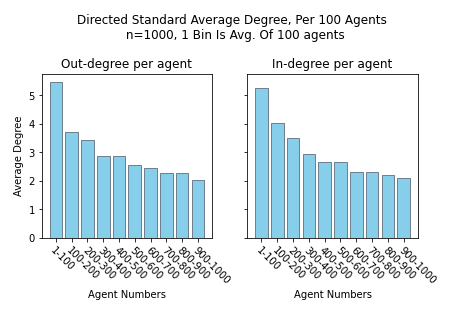
\includegraphics[width=.8\textwidth]{ThesisKI/Images/DirectedStandardPerAgent.png}
        \caption{Average Directed Degree}
        \label{degree:agent}
    \end{figure}
\end{center}

\noindent In this figure each bin represent the average degree over 100 agents, in order. It is clear that the earlier agents in the network tend to have a higher degree then later agents in the network, simulating this natural behaviour in the evolution of social groups. This benefit is lost when using the alternative method as there are no guaranteed links to earlier agents, removing this implicit bias.

\subsubsection{Customization}

As mentioned the chosen method has the option to adjust the generation process as desired. These adjustment are applied complementary to the default generation, to ensure the base guarantees of this method. \newline

First of all, this method allows for the generation of both directed and undirected networks. The method for generating undirected networks is very similar to the generation of directed networks. In fact, the process is entirely the same, save for one detail. In contrast to the generation of a directed network, where the agents to receive and send a link are chosen independently, and therefore tend to be distinct agents, the generation of an undirected network simply chooses one random agent to both receive and send a link. After all, the only difference between the interaction matrix $\T$ of a directed and undirected network is that the matrix of an undirected is symmetrical, whereas the matrix of an undirected network is asymmetrical. \newline
Furthermore, when a directed network is created it can be made into an undirected network. This can be done in one of three different ways. The first method is to duplicate all links, both the incoming and outgoing. This is done by simply taking the element wise maximum of the original matrix and its transpose, which effectively mirrors all links in the matrix along the diagonal. \newline

Secondly, the function also allows the choice of increasing the degree of each agent. The default generation guarantees each agent no more than one incoming and outgoing link. As this is sufficient to ensure connectedness, it does tend towards a lower amount of links per agent as shown in figure \ref{deg:std}, which shows the degree distribution of an undirected network, using the default generation. Furthermore the distribution has a sharp peak at the lower degrees, which quickly dissipates as the degree increases. In comparison, the degree distribution when using this increased degree becomes more spread out, over a wider range of degrees, and is flattened more.

\begin{figure}[!htbp]
  \centering
  \subfloat[Standard Degree]{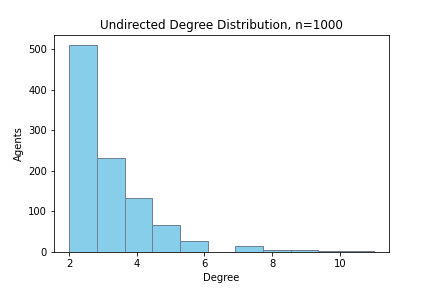
\includegraphics[width=0.5\textwidth]{ThesisKI/Images/DegreeUndirectedStandard.png}\label{deg:std}}
  \hfill
  \subfloat[Increased Degree]{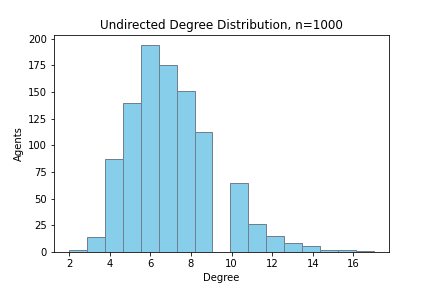
\includegraphics[width=0.5\textwidth]{ThesisKI/Images/DegreeUndirectedIncreased.png}\label{deg:inc}}
  \caption{Degree Distributions}
\end{figure}

\newpage

The implementation of this increased degree is rolled into the generation of the network to roll this functionality into the iteration of the generation function, preventing the need to repeat this iteration if the degree would be increased after the generation. After the guaranteed connections each agent then gets assigned an additional degree, which is a random number sampled from a given probability distribution, by default $\mathcal{N}(2,1)$. This number is rounded to the nearest integer. Subsequently, this amount of agents are down randomly from the set of \emph{all} agents in the network, and a link is created for those agents. When generating a directed network this procedure, including a random additional degree, occurs twice, once for the incoming degree, once for the outgoing degree. However, for an undirected network this procedure only needs to be executed once, and the chosen agents are used for both the incoming and outgoing link. \newline
The generation of this additional degree can customized further by providing a different probability function and the corresponding parameters. This allows for the degree to be increased as much as desired, using any probability distribution.\newline

Finally, the probability for self-links in the network can be set as desired. To guarantee that each agent in the network has a self-link this parameter can be set to 1 and, conversely, to ensure no agent \footnote{Except for the first agent, which always receives a self-link to ensure aperiodicity} has a self-link this parameter can simply be set to 0. Any value in between gives each agent that probability to have a self-link.

Below is an example of an undirected network generated using this method, with increased degree:
\begin{center}
    \begin{figure}[!htbp]
        \centering
        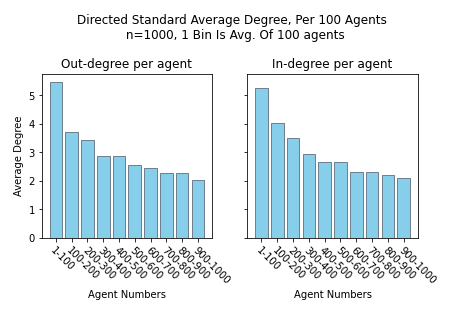
\includegraphics[width=.8\textwidth]{ThesisKI/Images/DirectedStandardPerAgent.png}
        \caption{Average Directed Degree}
        \label{degree:agent}
    \end{figure}
\end{center}

\newpage

\subsubsection{Sparse Matrices}

One caveat of the chosen method is the memory usage of matrices. As the interaction matrices are two-dimensional their memory usage increases quadratically as the network size increases. For small network this size this is negligible, however, as the sequences of networks grow towards the thousands of agents this becomes increasingly memory intensive. Therefore, in order to alleviate the intensive memory use of large matrices, the networks are generated as sparse matrices by default \cite{2020SciPy-NMeth}. As the generated network tend to contain only a small fraction of possible links the corresponding arrays will contain mainly zeros. However, it is not the lack of link that is of interest, but rather the presence of one, making all zero entries effectively a waste of space. Sparse matrices are created for this very purpose, increase memory efficiency of large arrays containing an overwhelming majority of empty data. The difference in memory usage is highlighted in figure \ref{generation:memory} below.

\begin{figure}[!htbp]
    \centering
    \subfloat[]{\label{generation:memory}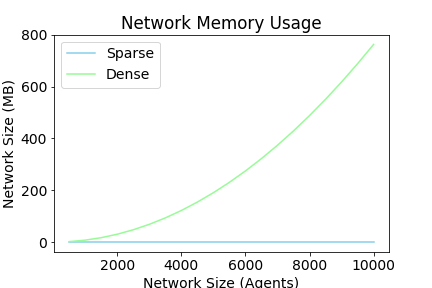
\includegraphics[scale=.45]{ThesisKI/Images/Memory.png}}
    
    \begin{minipage}{.5\linewidth}
    \centering
    \subfloat[]{\label{generation:time_inc}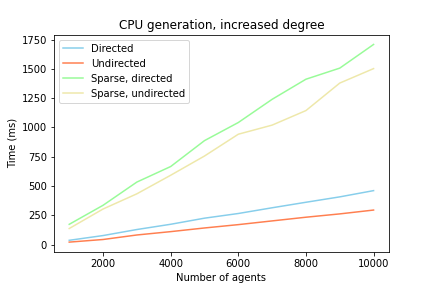
\includegraphics[scale=.4]{ThesisKI/Images/CPU_inc.png}}
    \end{minipage}%
    \begin{minipage}{.5\linewidth}
    \centering
    \subfloat[]{\label{generation:time_std}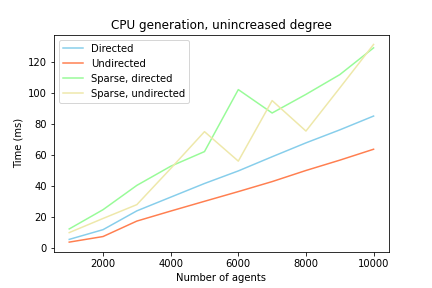
\includegraphics[scale=.4]{ThesisKI/Images/CPU.png}}
    \end{minipage}\par\medskip
    \caption{Network generation, \\ memory and time consumption}
\end{figure}

\newpage

While it is clear from the visualizations that the memory usage of sparse matrices, in this context, is an incredible improvement, it is not entirely without its downsides. As can be seen in figures \ref{generation:time_inc} and \ref{generation:time_std} sparse networks are slower to generate then their dense counterparts. However, the generation time for \emph{both} types still only increases linearly. As the generation time is only a one-time operation this difference can be considered negligible, making generation of networks using sparse networks the most beneficial default option.

\subsection{Fixed Generation}

Besides 

\section{Belief Initialization}

\section{Weight Initialization}
\subsection{Uniform}
\subsection{Overlap}
\subsection{Belief}
\subsection{Random}

\section{Non-cooperative Agents}

\section{Updating Rules}
\newpage
\section{Appendix}
\subsection{Proof of (strong) connectedness}
Let a network of containing 1 agent be our base case. This network is guaranteed to be fully connected, as the first agent is guaranteed to receive a self-link. Then assuming that we have an arbitrary network of size $n$, generated using the aforementioned method, that is strongly connected, when this network is extended to the size $n+1$, using the same method, it will also be strongly connected. Let $i$ be the $n+1$'th agent, that is to say, the agent added to the network to increase it in size. As the network is grown using the aforementioned method $i$ is guaranteed to have an incoming and outgoing link to the arbitrary agents $j < n+1$ and $k < n+1$. As $j < n+1$ and $k < n+1$ it follows naturally that $j, k \in \{1, ... n\}$, and are therefore agents in the network of size $n$. However, the network of size $n$ is strongly connected, so therefore there must exist some path to and from $j$ to and from any other agent in the network, as is the case for $k$. Therefore if $i$ has a link to both $j$ and $k$ there must also be a path to and from $i$ to and from every other agent in the network. Furthermore, as $j$ and $k$ were arbitrary, this holds for every agent $i$ is guaranteed to have a link with. Therefore the network of size $n+1$ is guaranteed to be strongly connected, if the aforementioned method of generation is used.\newline

\bibliographystyle{apalike}
\bibliography{references.bib}

\newpage
\end{document}